\documentclass{report}
\usepackage[margin=1.25in]{geometry}
\usepackage{hyperref}
\usepackage{amsmath}
\usepackage{amssymb}
\usepackage{amsthm}
\usepackage{listings}
\usepackage{parskip}
\usepackage{graphicx}
\usepackage[center]{caption}
\newtheorem{thm}{Theorem}
\title{Guidelines for the Creation of Readable Source Code}
\author{Varik Valefor}
\begin{document}
\maketitle{}
\tableofcontents{}
\chapter{WESTERNUNIONSOFTHECOUNTRYWESTERNS}
\begin{figure}
	\centering
	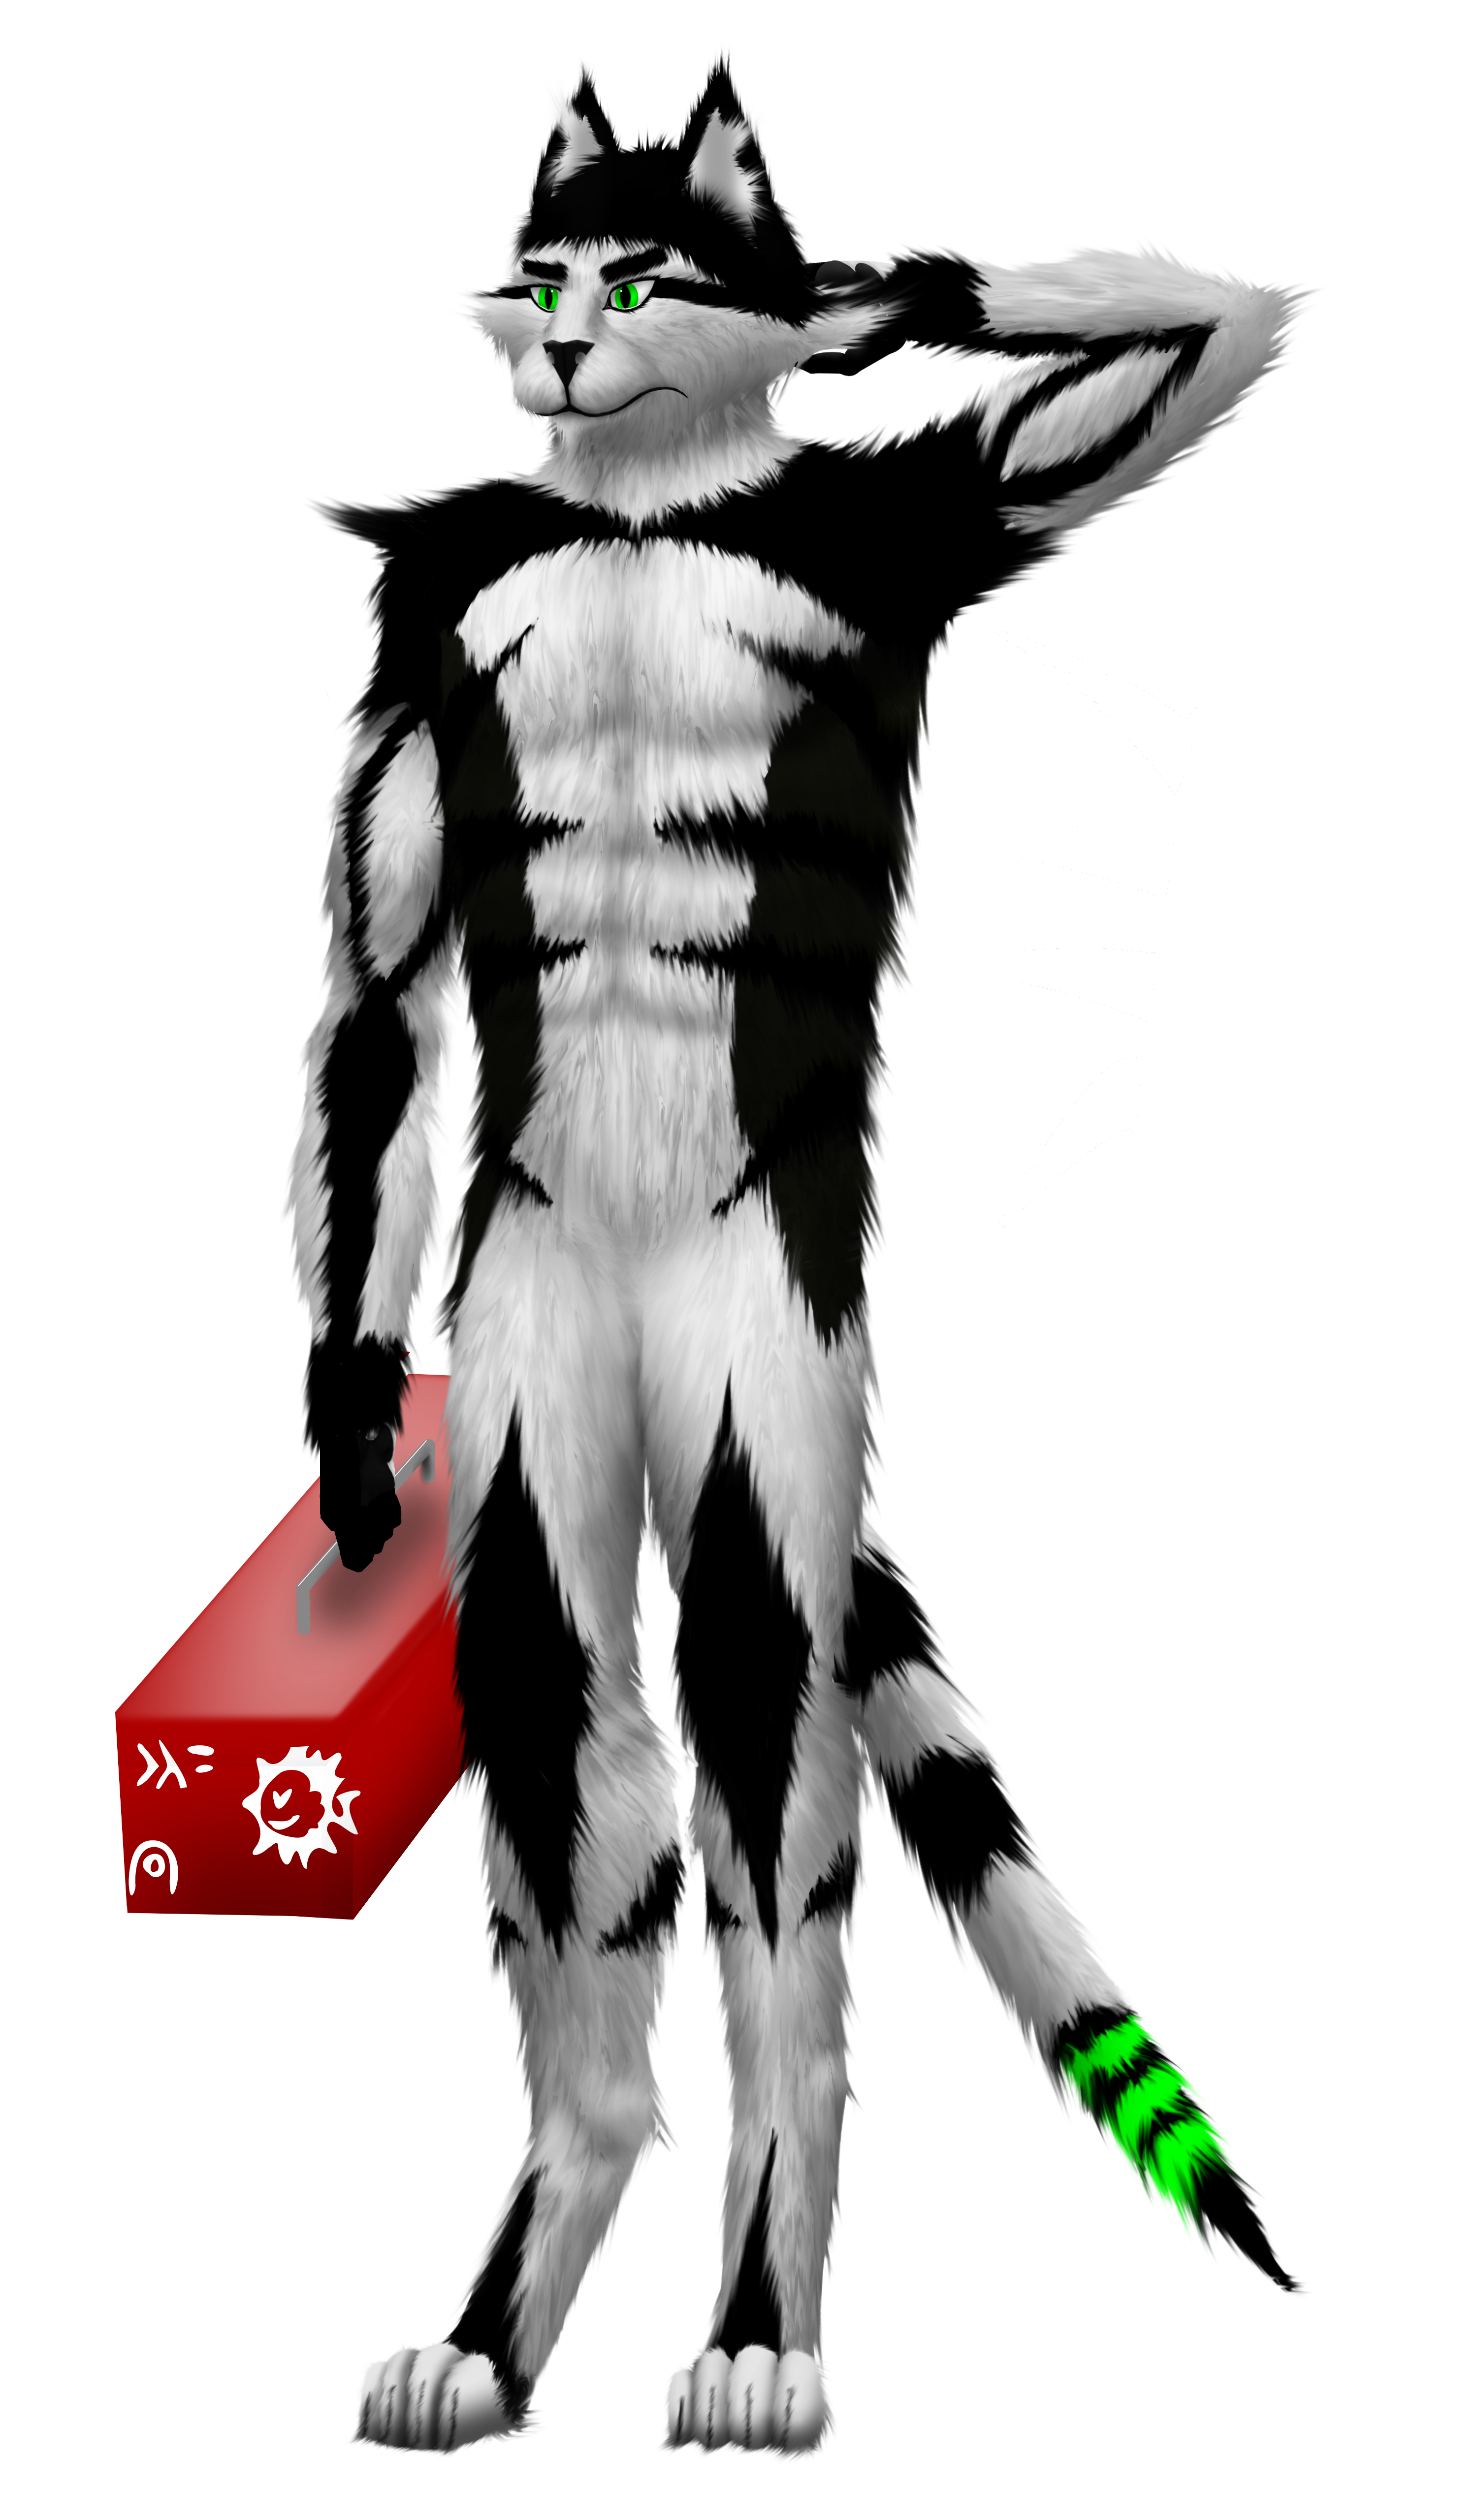
\includegraphics[height=10cm]{50x/toolbox/westernunionsofthecountrywesterns.png}
\caption{The actual drawing, as opposed to a bunch of text.}
\end{figure}
\section{The Original Description of the Drawing}
\subsection{A Successful ``Three-Quarters'' Thing}
After trying and struggling to draw VARIK's character in a ``three quarters'' pose for a decent period of time and taking rather long breaks between drawings, VARIK actually manages to somewhat decently draw VARIK's character such that VARIK's character is depicted in a ``three quarters'' pose.
\subsection{Watermarking and Licensing}
Additionally, this drawing is not \textit{too} obnoxiously watermarked.  However, this drawing is NOT released into the public domain.  VARIK retains the rights to this drawing, although this fact may change as time passes; as time passes, VARIK becomes increasingly friendly to the idea of releasing VARIK's drawings into the public domain.
\subsection{Tools Used}
This drawing is drawn using Krita, which VARIK quite dislikes.

During the creation of this drawing, Krita is all but unusably slow, as Krita manages to make layers invisible in the short timespan of approximately thirty seconds.  Partially as a result of this slowness, VARIK may create future drawings using CLIP STUDIO PAINT EX; VARIK owns a copy of CLIP STUDIO PAINT EX and finds that CLIP STUDIO PAINT EX is superior to Krita by nearly every metric.  VARIK's appreciation for WINE on FreeBSD manages to grow even greater.

GIMP is also used for a short while; however, after being in development for multiple decades, GIMP lacks some basic features which VARIK uses, e.g., clipping masks.  As such, VARIK completes this drawing with Krita.
\subsubsection{Yes, Open-Source Stuff \textit{can} be All Right}
The ``open-source'' idea is cool\ldots but can generate some real shit.  ``Critics can fix the software'' is a crap excuse, as not all users are computer programmers.  Additionally, nearly unmaintainable source code exists, and VARIK does not find that Krita's source code is particularly good.

These problems are mentioned because VARIK wishes to like Krita and GIMP\ldots but cannot actually like Krita and GIMP unless Krita and GIMP stop being frass.
\subsection{``Logos'' and Whatnot}
Determining the meanings of the ``logos'' which are present on the toolbox is left as a trivial exercise for the reader.  ``[L]ogos'' is written in inverted commas because some such things may not really be logos.
\subsection{On the Use of Version Control}
The history of this file may eventually be uploaded to GitHub; this file is tracked via Git, generating a fairly large repository.  However, this history \textit{may} be encrypted, as VARIK wishes to be able to reasonably easily provide evidence of VARIK's having created this drawing.
\subsection{Criticism}
As ever, decent criticism is strongly appreciated.  However, VARIK requests that such criticism is detailed; VARIK finds that the extent to which ``the shape of the fur does not match the shading of the arm'' is helpful is greater than the extent to which ``the fur looks bad'' is helpful, although both things can be helpful.
\subsection{Tools Used}
This description is written with the good ol' ed(1).

\chapter{HOLLYWOODFREAKSONTHEHOLLYWOODSCENE}
\begin{figure}
	\centering
	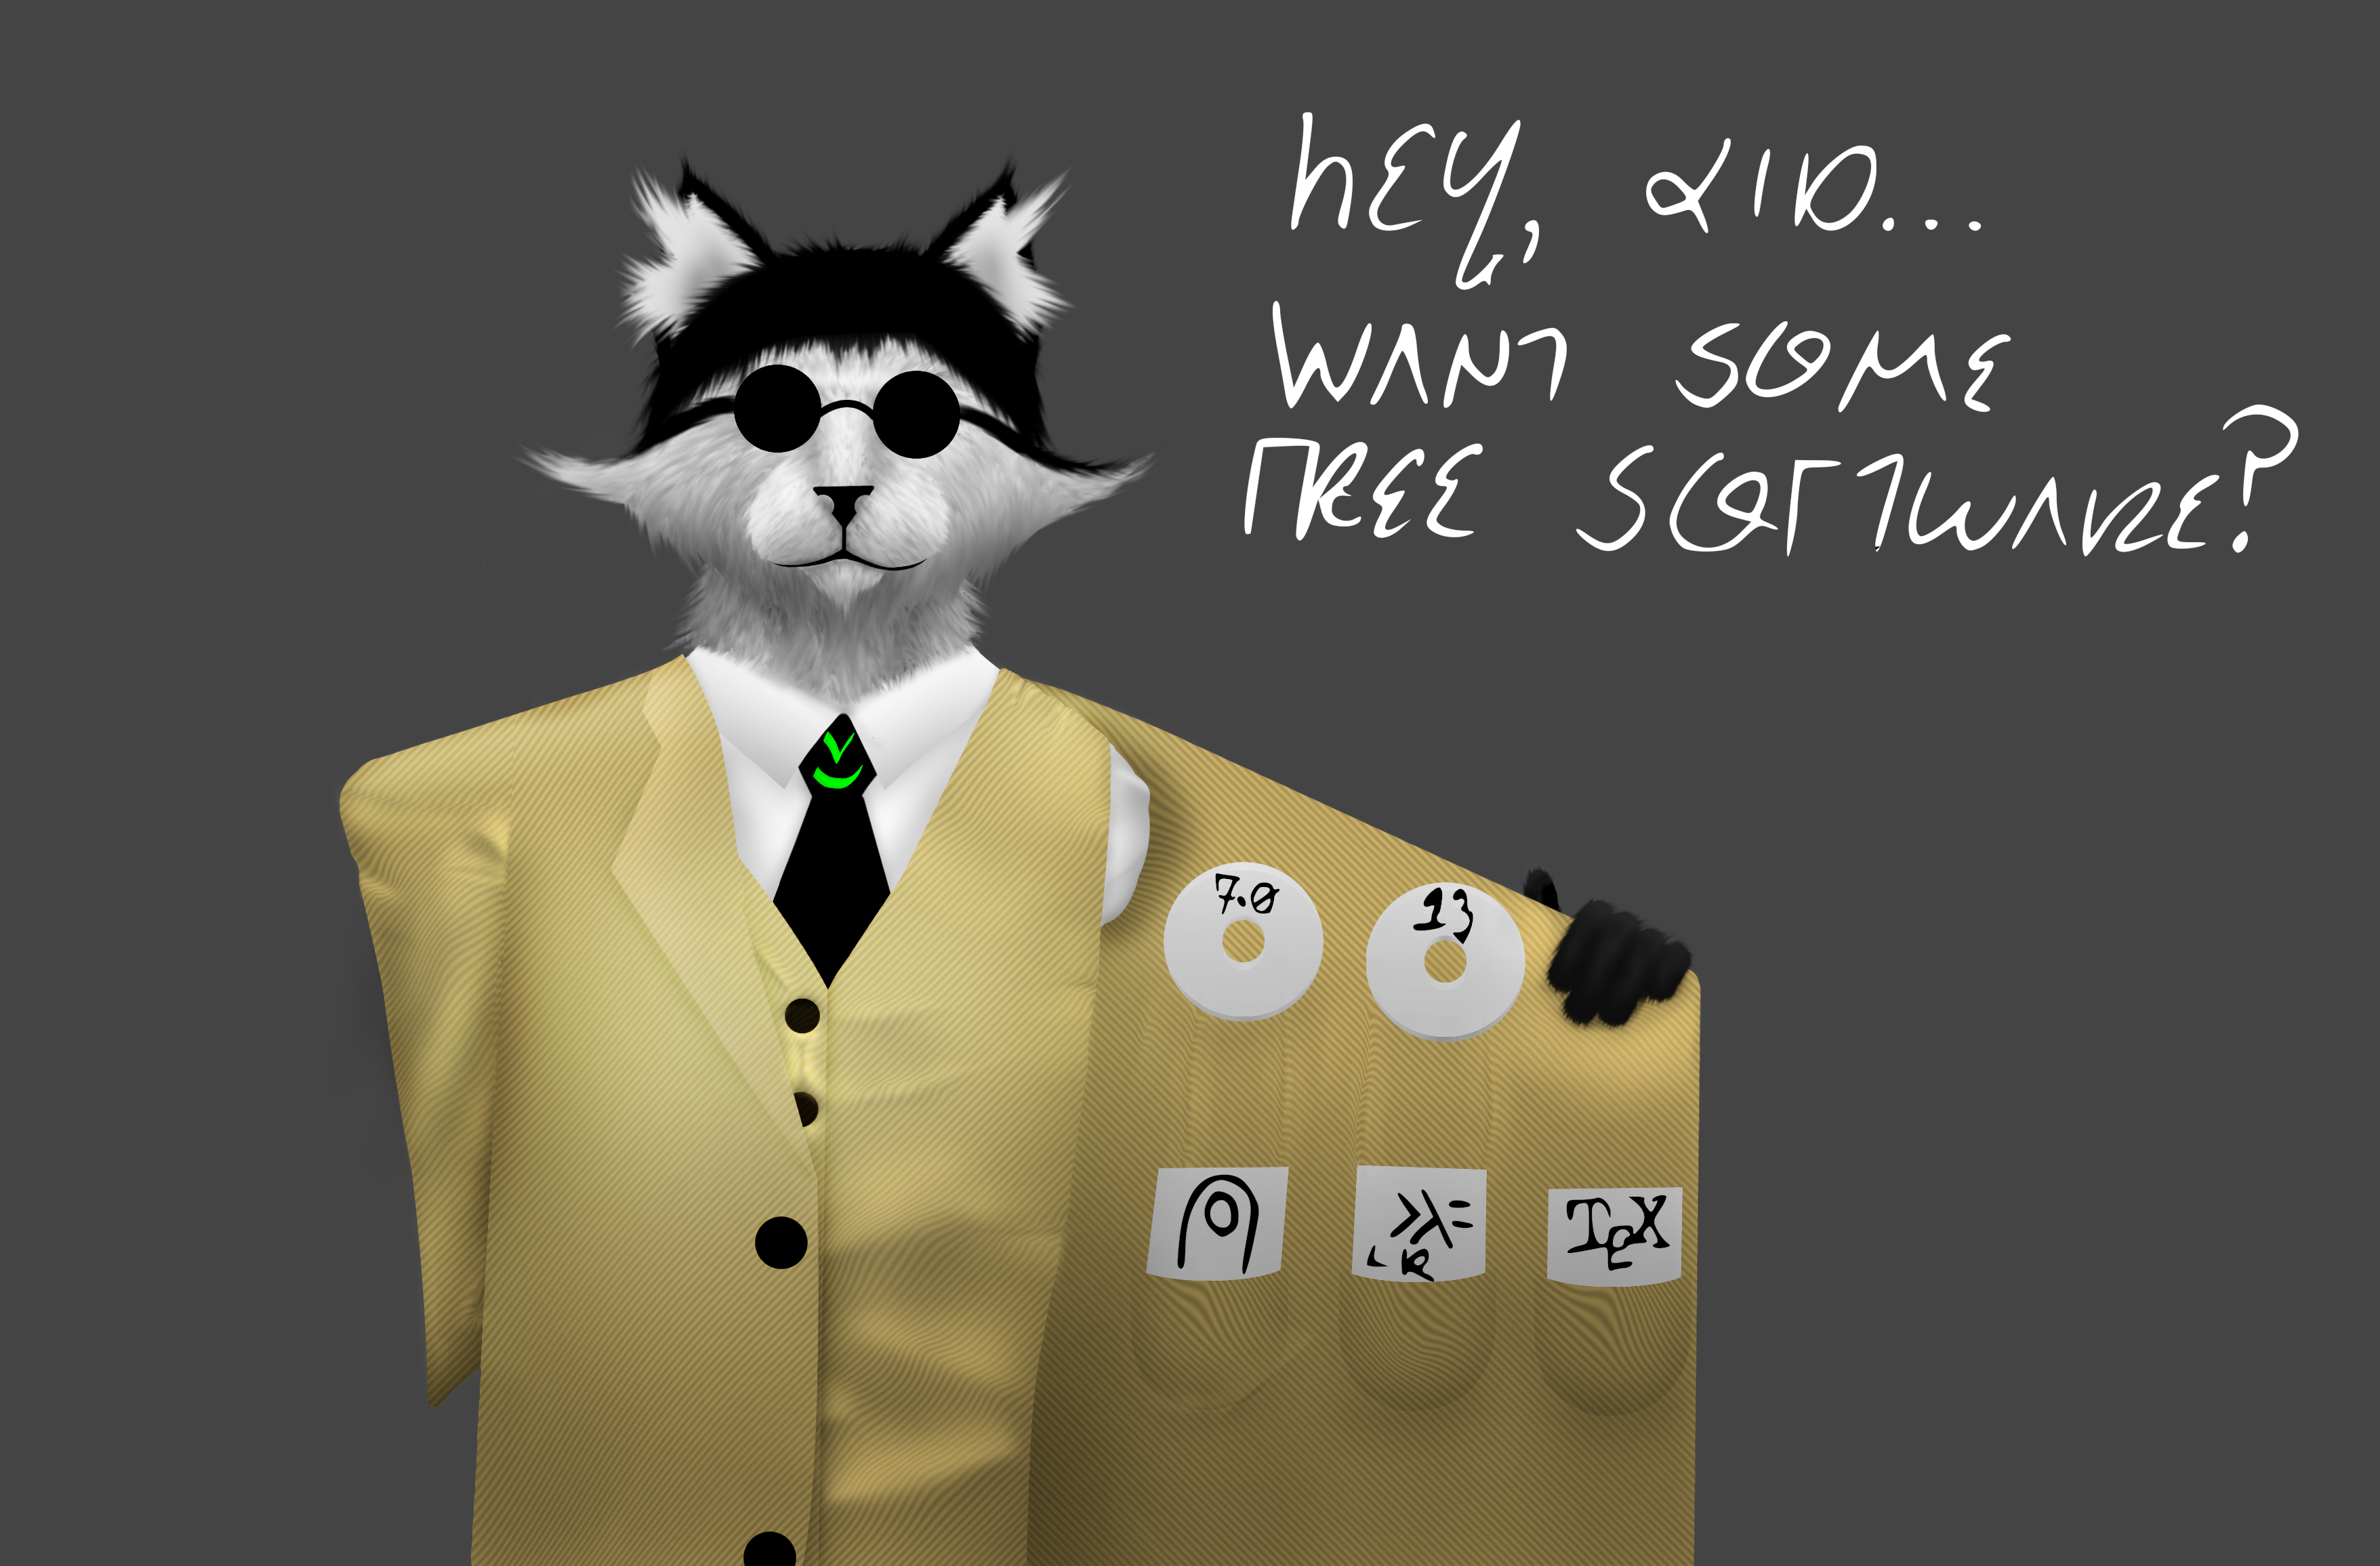
\includegraphics{hollywoodfreaksonthehollywoodscene/hollywoodfreaksonthehollywoodscene.png}
	\caption[center]{``HOLLYWOODFREAKSONTHEHOLLYWOODSCENE''.}
\end{figure}
\section{The Original Description of the Drawing}
\subsection{A Cheesy-Ass Short Story}
Let there exist a man $J$.

$K$ denotes the depicted man.

In the middle of an arbitrary night, as $J$ walks down an arbitrary street and nears a power substation, $K$ appears from behind a bush and slowly approaches $J$.

Whilst $J$ appears rather surprised and unnerved, $K$ opens $K$'s coat and speaks the following words: ``Hey, kid... want some free software?''

Determining whether or not $J$ ``takes up'' $K$'s offer is left as an exercise for the reader.
\subsection{Blah}
Another dumb joke is revealed!  In this case, the joke takes the form of a drawing which is called ``HOLLYWOODFREAKSONTHEHOLLYWOODSCENE''.

In addition to being a dumb joke, this drawing is VARIK's first \textit{real} attempt to draw fabric.
\subsection{The Contents of the Coat}
\subsubsection{Discs}
The ``7.0'' disc is an OpenBSD installation disc, and the ``13'' disc is a FreeBSD installation disc.  As of the publishing of this drawing, 7.0 and 13.0 are the most recent versions of OpenBSD and FreeBSD, respectively.
\subsubsection{Coat Pockets}
The reader can assume that the contents of the pockets of the coat are specifications and compilers of the programming languages whose ``logos'' are mentioned.  ``[L]ogos'' is written in inverted commas because one such ``logo'' is not an established logo but is a recognisable feature of the programming language which this ``logo'' represents.
\subsubsection{On the Amount of Stuff}
Whilst conceptualising this drawing, VARIK intends to mention a relatively great number of softwares.  However, there exists an idea such that this idea does not immediately come to fruition.  A ``deluxe'' version of this drawing may eventually be created.
\subsection{Criticism}
As ever, criticism regarding this drawing is appreciated.
\subsection{Tools Used}
This drawing is drawn using GIMP.

This description is written using ed(1).
\end{document}
